\documentclass[11pt,a4paper]{article}
\usepackage[top=21mm,bottom=21mm,left=22mm,right=22mm,headheight=15pt,headsep=7mm]{geometry}
\usepackage{fontspec}
\setmainfont{Cambria}
\setsansfont{Calibri}
\setmonofont{Consolas}[Scale=0.88]
\newfontfamily\banglafont{Nirmala UI}[Script=Bengali]
\usepackage{amsmath,amssymb,graphicx,xcolor,booktabs,tabularx,array,enumitem}
\usepackage{fancyhdr,titlesec,caption,float,microtype,tikz,tcolorbox}
\usetikzlibrary{arrows.meta,positioning,calc}
\usepackage{hyperref}
\definecolor{Ink}{HTML}{173047}
\definecolor{Blue}{HTML}{245878}
\definecolor{Ember}{HTML}{BC4221}
\definecolor{Mist}{HTML}{EEF4F7}
\definecolor{Muted}{HTML}{536575}
\definecolor{Rule}{HTML}{D4DFE6}
\color{Ink}
\hypersetup{colorlinks=true,linkcolor=Blue,urlcolor=Blue,citecolor=Blue,
  pdfauthor={Team KUETaguns},pdfsubject={NASA Space Apps project documentation, 29 October 2026},
  bookmarksnumbered=true,pdfdisplaydoctitle=true}
\urlstyle{same}
\setlength{\parindent}{0pt}
\setlength{\parskip}{6.5pt}
\linespread{1.075}
\setlength{\emergencystretch}{2em}
\raggedbottom
\widowpenalty=10000
\clubpenalty=10000
\titleformat{\section}{\Large\sffamily\bfseries\color{Ink}}{\textcolor{Ember}{\thesection}}{0.7em}{}
\titleformat{\subsection}{\normalsize\sffamily\bfseries\color{Blue}}{}{0em}{}
\titlespacing*{\section}{0pt}{0pt}{11pt}
\titlespacing*{\subsection}{0pt}{11pt}{4pt}
\captionsetup{font={small},labelfont={bf,sf},labelsep=period,skip=6pt}
\setlist[itemize]{leftmargin=1.4em,itemsep=3pt,topsep=3pt,parsep=0pt}
\setlist[enumerate]{leftmargin=1.7em,itemsep=5pt,topsep=4pt,parsep=0pt}
\newcolumntype{L}[1]{>{\raggedright\arraybackslash}p{#1}}
\newcolumntype{Y}{>{\raggedright\arraybackslash}X}
\renewcommand{\arraystretch}{1.19}
\setlength{\tabcolsep}{5pt}
\pagestyle{fancy}
\fancyhf{}
\fancyhead[L]{\small\sffamily\textbf{AGUN PANJIKA}}
\fancyhead[R]{\small\sffamily\color{Muted}\ReportShortTitle}
\fancyfoot[L]{\footnotesize\sffamily\color{Muted}KUETaguns\enspace|\enspace 29 October 2026}
\fancyfoot[R]{\footnotesize\sffamily\thepage}
\renewcommand{\headrulewidth}{0.4pt}
\renewcommand{\footrulewidth}{0pt}
\newcommand{\ReviewDate}{29 October 2026}
\newcommand{\Repo}{https://github.com/polymathicX/Agun-Panjika}
\newcommand{\RepoLink}[2]{\href{https://github.com/polymathicX/Agun-Panjika/blob/main/#1}{#2}}
\newcommand{\SourceNote}[1]{{\small\color{Muted}#1}\par}
\newcommand{\ReportPage}[2]{\clearpage\section{#1}\label{#2}}
\newcommand{\Eyebrow}[1]{{\small\sffamily\bfseries\color{Ember}\MakeUppercase{#1}}\par}
\newenvironment{keypoint}[1]{\begin{tcolorbox}[colback=Mist,colframe=Rule,boxrule=0.5pt,
  arc=1mm,left=3mm,right=3mm,top=2mm,bottom=2mm]
  {\sffamily\bfseries\color{Blue}#1}\par\smallskip}{\end{tcolorbox}}
\newcommand{\Metric}[2]{\begin{minipage}[t]{.31\linewidth}\sffamily\raggedright
  {\fontsize{25}{27}\selectfont\bfseries\color{Blue}#1}\par
  \vspace{3pt}{\small\color{Muted}#2}\end{minipage}}
\newcommand{\CoverRule}{\par\vspace{4mm}{\color{Ember}\rule{24mm}{1.2pt}}\par\vspace{5mm}}
\tikzset{box/.style={draw=Rule,fill=Mist,rounded corners=2pt,align=center,
  font=\sffamily\small,inner sep=6pt,text=Ink},
  arrow/.style={-{Stealth[length=2mm]},draw=Blue,line width=.7pt}}

\newcommand{\ReportShortTitle}{Project brief for academic review}
\hypersetup{pdftitle={Agun Panjika: Project Brief for Academic Review}}
\begin{document}
\thispagestyle{empty}
\Eyebrow{NASA Space Apps Challenge 2026}
\vspace{6mm}
{\fontsize{34}{38}\selectfont\sffamily\bfseries Agun Panjika}\par
{\Large\banglafont আগুন পঞ্জিকা}\par
\vspace{3mm}
{\Large\sffamily Project brief for academic review}\par
\CoverRule
{\large A comparable fire history.\quad A clearer view of the season.}\par
\vspace{4mm}
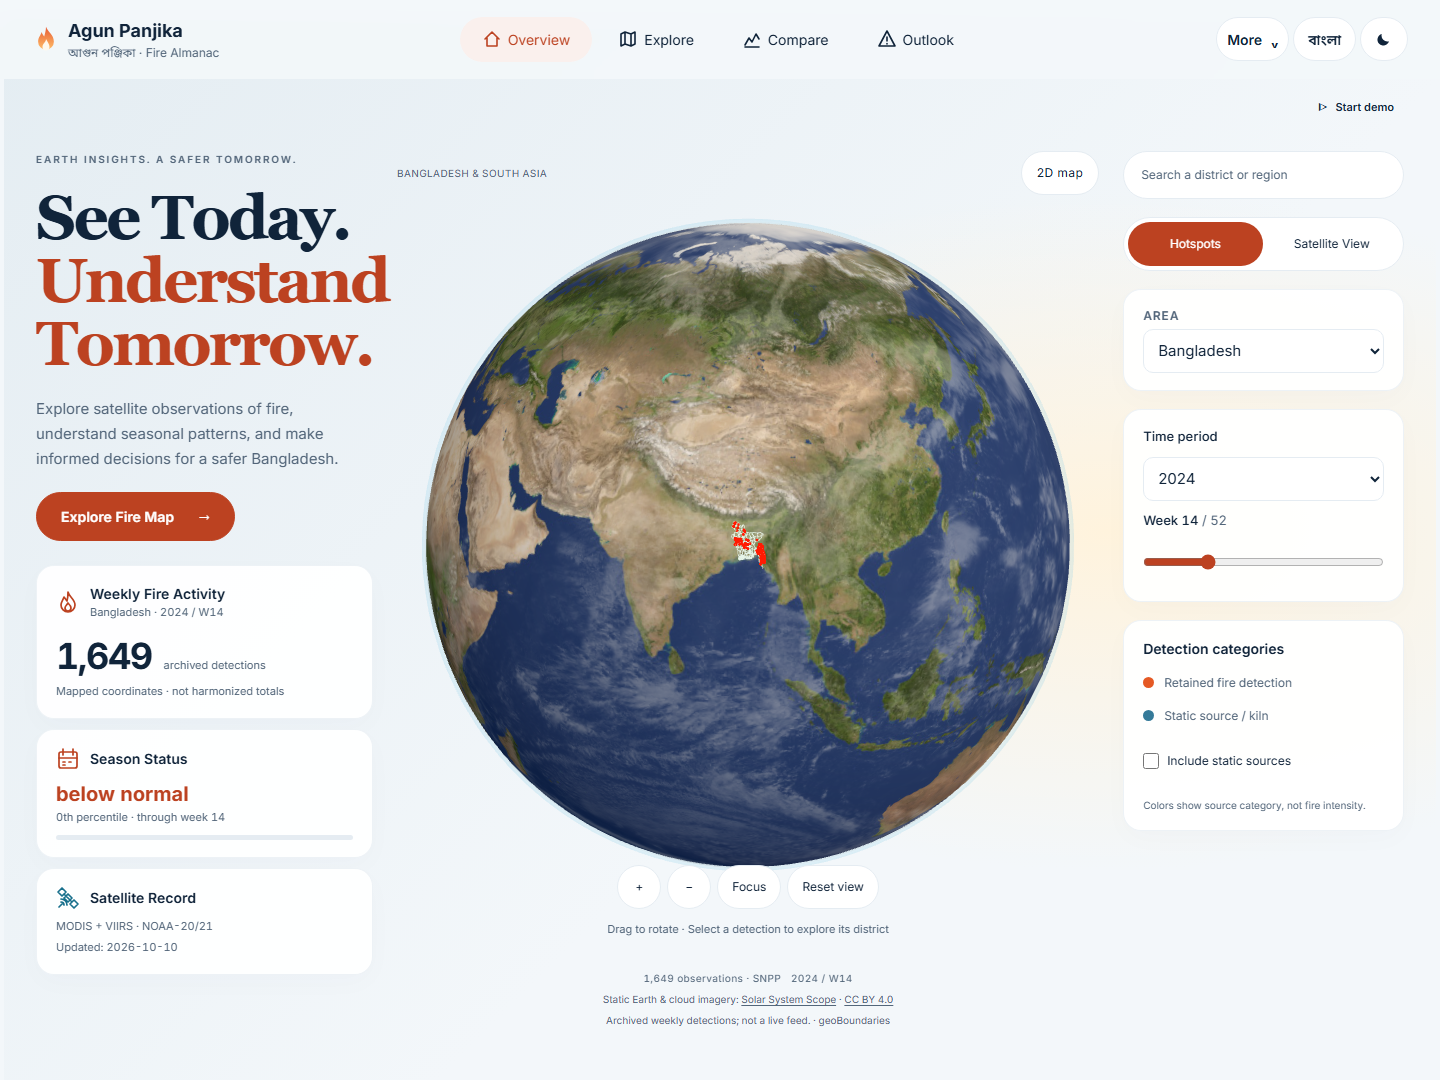
\includegraphics[width=\linewidth]{../review/screenshots/home-desktop.png}
\vspace{4mm}
{\sffamily\bfseries Team KUETaguns}\par
Khulna University of Engineering \& Technology (KUET), Bangladesh\par
\small Harmonization of MODIS and VIIRS Hot Spots\par
\vfill
\begin{minipage}[t]{.56\linewidth}
\small\textbf{Prepared for mentorship and research discussion}\par
Reviewed \ReviewDate.\par
Data snapshot: \mbox{9 October 2026}.
\end{minipage}\hfill
\begin{minipage}[t]{.38\linewidth}\small\raggedleft
\href{\Repo}{Source code and documentation}\par
\href{https://youtu.be/9FMIzcXhqB4}{Project video}\par
\RepoLink{docs/GLOBAL_EXTENSION_PLAN.md}{Global extension proposal}
\end{minipage}

\ReportPage{Executive overview}{sec:overview}
\begin{keypoint}{The question the project helps a user investigate}
\large\textbf{Is this fire season normal for this area?}
\end{keypoint}
Agun Panjika (Fire Almanac) is an English/Bangla web application and a Python pipeline for comparing Bangladesh's satellite-detected fire activity across changes in observing instruments. It starts with Bangladesh, particularly the Chittagong Hill Tracts, and is intended for forest officers, communities, researchers and newsrooms.

\subsection{Why harmonization is necessary}
MODIS and VIIRS observe at different spatial resolutions and sensitivities. NASA FIRMS provides MODIS active-fire layers at approximately 1\,km and VIIRS at 375\,m. Joining their raw counts can make an instrument change look like a change in burning. Those resolutions describe observations, not the size or number of unique fires.

The pipeline reconstructs earlier weekly activity on a VIIRS S-NPP detection scale, distinguishes observed and estimated periods, and exposes uncertainty. The interface connects that comparable history to calendars, maps, seasonal normals and shareable reports.

\vspace{3mm}
\Metric{2001 onward}{Historical record, with early periods reconstructed}\hfill
\Metric{64 districts}{Five analysis regions across Bangladesh}\hfill
\Metric{25.25\%}{Lower internal weekly MAE than a fitted factor}
\vspace{5mm}

\subsection{What the current evidence supports}
The committed internal leave-one-year-out evaluation for 2012--2025 reports national weekly mean absolute error (MAE) of 36.964 detections, versus 49.450 for a single factor fitted within each training fold. This is a promising reconstruction benchmark, not an independently confirmed final result or operational forecast accuracy.

The software is a working prototype. The 29 October checks passed 59 Python tests, typechecking, the production build and eleven browser test groups covering 42 route/theme/language/viewport views. A field-user study, prospective warning evaluation and reliable hosted refresh have not been established.

\begin{keypoint}{Purpose of academic mentorship}
The immediate need is to strengthen evaluation independence, position the contribution against prior work, and decide whether the next milestone should be a deeper Bangladesh user pilot or an independently evaluated transfer case.
\end{keypoint}

\subsection{Reading guide}
Data and product: page~\pageref{sec:data}. Method and architecture: page~\pageref{sec:method}. Internal results: page~\pageref{sec:results}. Continuity and outlooks: page~\pageref{sec:continuity}. Verification and limitations: page~\pageref{sec:limits}. Research questions and evidence links: page~\pageref{sec:agenda}.

\ReportPage{Data, geography and implemented product}{sec:data}
\subsection{Data provenance}
\begin{table}[H]\small
\begin{tabularx}{\linewidth}{@{}L{31mm}YY@{}}
\toprule
\textbf{Source} & \textbf{Role in the project} & \textbf{Interpretation limit}\\\midrule
NASA FIRMS & MODIS Terra/Aqua; VIIRS S-NPP, NOAA-20 and NOAA-21 observations & A detection is not a unique fire; omissions and repeat observations remain possible.\\
NASA POWER & Historical weather, FWI inputs and Dhaka aerosol context & Regional sampled/reanalysis context, not local station observations.\\
Open-Meteo & Forecast weather for experimental danger views & Actual forecast-feed skill needs prospective evaluation.\\
geoBoundaries & District/upazila assignment and administrative maps & Boundary versions and snapping influence local interpretation.\\
ESA Fire\_cci & Burned-area cross-check: MRBA v6.0, then Sentinel-3 SYN v1.1 & Different observable and a product change in 2019.\\
NOAA CPC ONI & Experimental ENSO covariate & Inclusion in an experiment does not establish improved skill.\\\bottomrule
\end{tabularx}
\caption{Data sources and their roles. Full attribution is linked on page~\pageref{sec:agenda}.}
\end{table}

\subsection{What is in the saved snapshot?}
The national record contains 1,345 ISO weeks from 2001-W01 through 2026-W41: 576 estimated and 769 observed. No successor-bridged week is present in that saved record. Observations end on \textbf{9 October 2026}; exports were generated on 10 October. The historical-normal baseline is 2003--2025. The saved weather forecast ends on 25 October, so the outlooks are archived examples as of this review.

The five analysis regions are Rangamati, Khagrachhari, Bandarban, Chattogram/Cox's Bazar hills, and the rest of Bangladesh. Local calendars cover 25 upazilas and 124 unions in the three CHT districts: Rangamati 10/51, Khagrachhari 8/41 and Bandarban 7/32. Earlier local values are apportioned estimates, not independently fitted local forecasts. Union names still need full Bangla localization and community review.

\subsection{Implemented user experience}
The seven routes provide an overview, fire calendar, sensor comparisons, map, experimental outlook, cross-border context and methodology. Users can inspect raw/factor/harmonized series, uncertainty, district patterns, archived point coordinates and seasonal percentiles; export CSV/PNG/print reports; or follow a bilingual guided demonstration.

The restored \textbf{Soft Earth} homepage uses a textured Three.js globe with linked area/year/week controls and a 2D fallback. The Earth/cloud textures are static geographic context. Shared URL state, mobile layouts, keyboard/table alternatives, loading/error/retry handling and cached offline access are implemented. External map tiles/fonts and unvisited resources are outside the offline guarantee.

\ReportPage{Method and system design}{sec:method}
\subsection{From observations to comparable weekly history}
The pipeline normalizes FIRMS metadata, removes exact duplicates, tags geography and filters confidence/type. It retains MODIS confidence at least 30\% and VIIRS nominal/high observations; excludes FIRMS static-land/offshore types; and uses persistence, day/night and seasonality to flag probable industrial heat cells. District-week counts, radiative power and sensor-composition features are aggregated to regions and the nation.

\begin{figure}[H]\centering
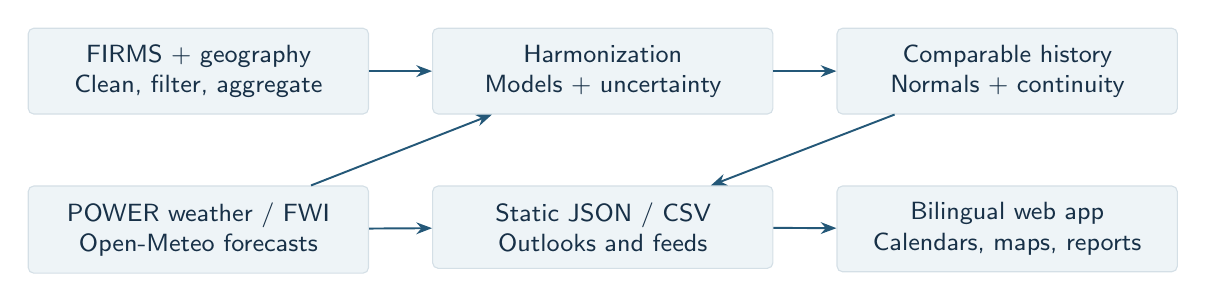
\begin{tikzpicture}[node distance=8mm]
\node[box,text width=39mm] (i) {FIRMS + geography\\Clean, filter, aggregate};
\node[box,text width=39mm,right=8mm of i] (h) {Harmonization\\Models + uncertainty};
\node[box,text width=39mm,right=8mm of h] (c) {Comparable history\\Normals + continuity};
\node[box,text width=39mm,below=9mm of i] (p) {POWER weather / FWI\\Open-Meteo forecasts};
\node[box,text width=39mm,below=9mm of h] (e) {Static JSON / CSV\\Outlooks and feeds};
\node[box,text width=39mm,below=9mm of c] (w) {Bilingual web app\\Calendars, maps, reports};
\draw[arrow] (i)--(h);\draw[arrow] (h)--(c);
\draw[arrow] (p)--(h);\draw[arrow] (c)--(e);\draw[arrow] (p)--(e);\draw[arrow] (e)--(w);
\end{tikzpicture}
\caption{Implemented data flow. ESA burned area supplies a separate external cross-check.}
\end{figure}

\subsection{Reconstruction model}
During the 2012--2025 overlap, regional weekly S-NPP counts are the target. A negative-binomial model uses MODIS count/FRP with regional and seasonal intercepts. Bagged Poisson LightGBM adds sensor composition, neighbouring-week counts, cloud/weather/FWI and viewing geometry. The shipped point estimate is
\begin{equation}
\widehat V_{r,w}=0.30\,\widehat V_{\mathrm{NB},r,w}
 +0.70\,\frac{1}{5}\sum_{s=1}^{5}\widehat V_{\mathrm{GBM},s,r,w}.
\end{equation}
Here $r$ is region, $w$ is week and $s$ indexes five model seeds. A separate, lower-confidence Terra-only reconstruction covers 2001 through 2002-W26. Some features include \textbf{next-week MODIS counts}: this is retrospective reconstruction, not an issue-time prediction algorithm.

\subsection{Uncertainty, continuity and season status}
Nominal 80\% intervals use held-out log-error distributions by activity/season, with separate annual-error treatment. Strictly nested calibration has not yet been established. Successor comparisons evaluate identity, fitted-factor and shrunk monthly corrections; both currently select identity. Season status ranks cumulative activity against complete historical years, excluding the displayed year.

Python prepares static exports; React/TypeScript/Vite consumes them without an application backend or database. D3 powers charts and the Canvas fallback, Three.js the textured Earth, and MapLibre the map. The pipeline/model code and exported evidence remain available for inspection.

\ReportPage{Internal reconstruction results}{sec:results}
The committed evaluation leaves out one overlap year at a time and compares national weekly predictions with S-NPP. The values below are means across held-out years over 2012--2025; no models were retrained for this report.

\begin{figure}[H]\centering
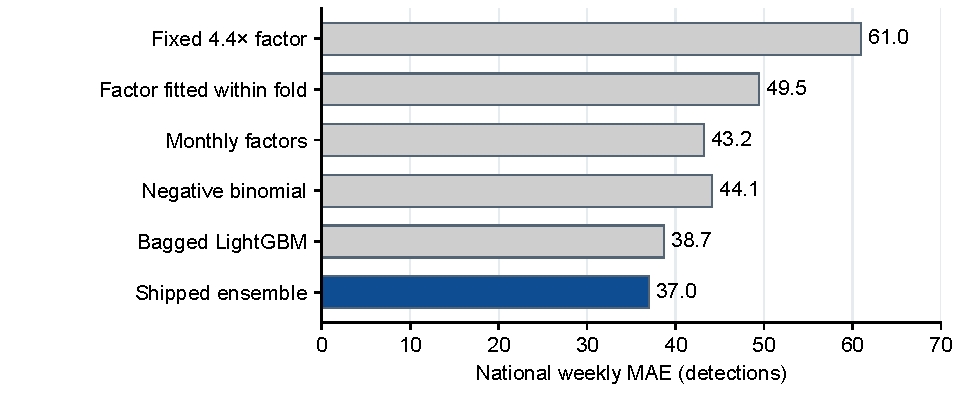
\includegraphics[width=\linewidth]{figures/model-comparison.pdf}
\caption{Internal national weekly MAE. Lower is better. Aggregate bars have no newly estimated confidence intervals.}
\end{figure}

\begin{table}[H]\small
\begin{tabularx}{\linewidth}{@{}Yrrr@{}}
\toprule
\textbf{Method} & \textbf{Weekly MAE} & \textbf{Off-season MAE} & \textbf{Annual error}\!\\\midrule
Fixed 4.4$\times$ factor &60.971&26.095&20.150\%\\
Factor fitted within fold &49.450&28.705&12.785\%\\
Monthly factors &43.180&21.933&11.888\%\\
Negative binomial &44.110&19.458&9.652\%\\
Bagged LightGBM &38.684&\textbf{15.347}&10.426\%\\
Shipped ensemble &\textbf{36.964}&15.861&\textbf{9.501\%}\\\bottomrule
\end{tabularx}
\caption{National errors from the saved validation export. Annual error is mean absolute annual-total percentage error; weekly MAE is measured in detections.}
\end{table}

The ensemble reduces weekly MAE by \textbf{25.25\%} against the fitted factor and 39.37\% against fixed 4.4$\times$. It beats the fitted factor in all 14 evaluated off-seasons. LightGBM alone has the lowest overall off-season MAE; the ensemble does not win every metric, region or year.

\begin{keypoint}{Uncertainty is material, not decorative}
Reported coverage is 80.1\% for region-weeks, 81.3\% for national weeks and 85.7\% for national years, against an 80\% target. Median national-week interval width is 1.39 times the estimate. Coverage should be interpreted alongside the calibration-independence concern.
\end{keypoint}

\SourceNote{Evidence: \RepoLink{web/public/data/validation.json}{validation.json}. The Terra-only model reports weekly MAE 66.76 versus 99.58 for a Terra scaling factor, with lower confidence in the earliest reconstruction. These are internal results, not an untouched final evaluation.}

\ReportPage{Continuity checks and experimental outlooks}{sec:continuity}
\subsection{An independent observable}
ESA burned area provides a plausibility check on annual/seasonal variability. The saved transition diagnostic is 0.95 for harmonized detections versus 3.09 for a raw stitched record; estimated-years log-annual correlation is 0.93 and seasonal-cycle correlation 0.98.

\begin{figure}[H]\centering
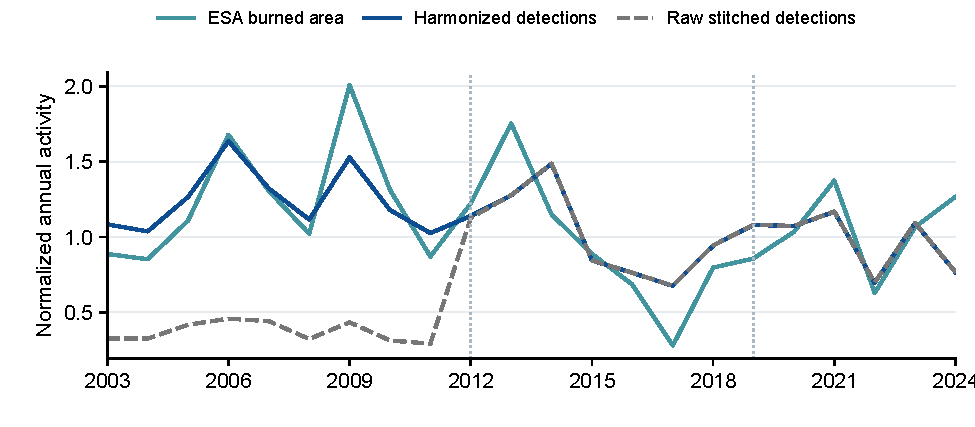
\includegraphics[width=\linewidth]{figures/continuity-crosscheck.pdf}
\caption{Annual series divided by their own 2012--2024 means. Markers identify VIIRS entry (2012) and the ESA product change (2019). Burned area and detection counts are different observables; agreement does not establish ground-truth fire-count accuracy.}
\end{figure}

\subsection{Successor-satellite continuity}
The selected identity bridge reports mean absolute held-out total errors of \textbf{4.58\% for NOAA-20} and \textbf{10.79\% for NOAA-21}. NOAA-21 has a shorter overlap including partial years. These results do not establish interchangeability in every district/season. Handover tests must cover main, local, neighbour and point products, missing observations and future nonidentity factors.

\subsection{Two-week activity outlooks}
\begin{table}[H]\small
\begin{tabularx}{\linewidth}{@{}Yrr@{}}
\toprule
\textbf{Hindcast setting} & \textbf{Brier skill} & \textbf{ROC AUC}\\\midrule
Fire history only &0.110&0.708\\
Fire history + observed future FWI &0.213&0.768\\\bottomrule
\end{tabularx}
\caption{Saved two-week hindcasts against climatology. The stronger weather experiment assumes access to future observed FWI.}
\end{table}

The weather-assisted result is an optimistic sensitivity experiment, \textbf{not actual forecast-feed accuracy}. End-to-end temporal separation and independent forecast calibration remain unestablished. The remainder-of-season product reports no sufficient skill and shows the normal range. Cross-border/aerosol views are exploratory associations, not a causal smoke-arrival model.

\SourceNote{Evidence: \RepoLink{web/public/data/partner.json}{partner.json}, \RepoLink{web/public/data/bridge.json}{bridge.json} and \RepoLink{web/public/data/forecast.json}{forecast.json}.}

\ReportPage{Verification, reproducibility and limitations}{sec:limits}
\begin{table}[H]\small
\begin{tabularx}{\linewidth}{@{}L{46mm}Y@{}}
\toprule
\textbf{Check on 29 October} & \textbf{Observed result and scope}\\\midrule
Python tests &59 passed; no skips in the available local environment.\\
TypeScript and production build &Passed for the restored Soft Earth interface.\\
Production browser regression &11 groups passed; 42 views with no recorded page/console errors, overflow or axe findings.\\
Visual restoration &Desktop screenshot matches the saved Soft Earth reference byte-for-byte; mobile view inspected.\\
Scientific regeneration &Not performed for this documentation; saved results were inspected.\\\bottomrule
\end{tabularx}
\caption{Software checks establish behavior under the tested setup. They are not field-user validation, full accessibility certification or a new scientific evaluation.}
\end{table}

\subsection{Research and release limits}
\begin{enumerate}
\item \textbf{Independent evaluation.} Some calibration residuals come from models that can include the evaluation year in training. Model/feature/weight selection and all learned preprocessing need separation from an untouched final holdout.
\item \textbf{Coverage and issue-time availability.} Reconstruction uses following-week information; forecast hindcasts consume an already-reconstructed record. Missing acquisition coverage must be distinguished from genuine zero activity.
\item \textbf{Static filtering and small areas.} The tuned filter's final image sample has 16 positive industrial labels out of 20; it is not an independent precision/recall study. District/local apportionment does not establish small-area calibration.
\item \textbf{Users and operational impact.} The five-person protocol has uncompleted rows. Native Bangla/CHT review, uncertainty comprehension and workflow fit need actual users. No field adoption, fires prevented or operational warning authority is claimed.
\item \textbf{Release readiness.} A working public app URL was not verified; hosted refresh had failed. Stale-product handling, dependency advisories, explicit software licensing and in-app method-copy drift remain follow-up work.
\end{enumerate}

\subsection{Reproduce the prototype and inspect the science}
Existing exports are enough to run the interface without a FIRMS key. Use \texttt{npm ci}, \texttt{npm run typecheck} and \texttt{npm run build} from \texttt{web/}. Python installation uses \texttt{python -m pip install -e ".[dev]"}; run \texttt{python -m pytest -q} from the root.

Full pipeline regeneration downloads inputs and fits models; inspect \texttt{python -m pipeline.run\_all --help} first. Keep API credentials in the gitignored pipeline environment. Record data/configuration versions, seeds and output hashes for new experiments.

\SourceNote{Instructions and provenance: \RepoLink{docs/VERIFICATION.md}{verification report}, \RepoLink{docs/review/verification-2026-10-29.json}{machine-readable checks}, \RepoLink{notebooks/validation.ipynb}{validation notebook} and \RepoLink{docs/SCIENTIFIC_REVIEW.md}{source-level scientific review}.}

\ReportPage{Research agenda and evidence index}{sec:agenda}
\subsection{Specific requests for academic guidance}
\begin{enumerate}
\item \textbf{Evaluation independence.} Which temporal/geographic splits, nested calibration and locked final holdout would make the main harmonization result defensible?
\item \textbf{Contribution and related work.} Which prior sensor-fusion methods, strong baselines and ablations should frame this system's contribution? The project uses established models rather than claiming a new foundational algorithm.
\item \textbf{Transfer.} Should the next milestone be a deeper Bangladesh case or a validated second-country demonstration? Which contrasting setting would test the method meaningfully?
\item \textbf{Practical use.} Which forest/community decision should the interface support? A domain reviewer and practitioner introductions would help shape a credible pilot.
\item \textbf{Research potential.} After the missing experiments, is there a focused paper or technical-report question? Publishability is an open question, not an assumed outcome.
\end{enumerate}

\subsection{Claim-to-evidence check}
\begin{table}[H]\small
\begin{tabularx}{\linewidth}{@{}L{46mm}Y@{}}
\toprule
\textbf{Claim} & \textbf{Current assessment}\\\midrule
Working bilingual prototype &Supported in the tested local environment by source, production captures and regression checks.\\
Lower reconstruction error &Supported as an internal benchmark; needs independent final confirmation.\\
Sensor continuity &Limited aggregate diagnostics support plausibility, not a bias-free or ground-truth record.\\
Guaranteed uncertainty, worldwide accuracy or operational impact &Not established; requires new evaluation and user evidence.\\\bottomrule
\end{tabularx}
\end{table}

\subsection{Selected sources and supporting materials}
\begin{itemize}\small
\item \href{https://firms.modaps.eosdis.nasa.gov/mapserver/wms-info/}{NASA FIRMS data/layer documentation}; \href{https://power.larc.nasa.gov/}{NASA POWER}; \href{https://climate.esa.int/en/projects/fire/}{ESA Fire\_cci}; \href{https://www.geoboundaries.org/}{geoBoundaries}; \href{https://open-meteo.com/}{Open-Meteo}.
\item \href{https://www.mdpi.com/2073-4433/14/1/97}{Farukh, Islam \& Hayasaka (2023), Atmosphere 14(1):97}: Bangladesh fire-season context, distinct from this project's validation.
\item \RepoLink{docs/SOURCES_AND_SUBMISSION.md}{Full source/imagery credits and submission notes}. Solar System Scope Earth/cloud textures are used under CC BY 4.0; basemap and imagery attributions remain in the app/repository.
\item \RepoLink{docs/PROJECT_BRIEF.md}{Detailed Markdown project brief}; \RepoLink{docs/GLOBAL_EXTENSION_PLAN.md}{global extension plan}; \href{https://youtu.be/9FMIzcXhqB4}{team video}; \href{\Repo}{source repository}.
\end{itemize}

\begin{keypoint}{Proposed outcome of the first mentor discussion}
Agree on one primary user journey, an independent evaluation protocol and the next bounded deliverable. The companion extension proposal gives milestones and acceptance criteria for that decision.
\end{keypoint}
\end{document}
